\documentclass[../main/main.tex]{subfiles}

\newdate{date}{11}{11}{2020}

% \begin{figure}[h!]
% \centering
% \includegraphics[page=6,width=0.8\textwidth]{../lessons/pdf_file/16_lecture.pdf}
% \end{figure}

%\displaydate{date}. Compiled:  \today. Alice.

\begin{document}

\pagestyle{plain}

\section{Lecture 16}


\subsubsection*{Slide 1}

\begin{minipage}[]{0.5\linewidth}
\centering
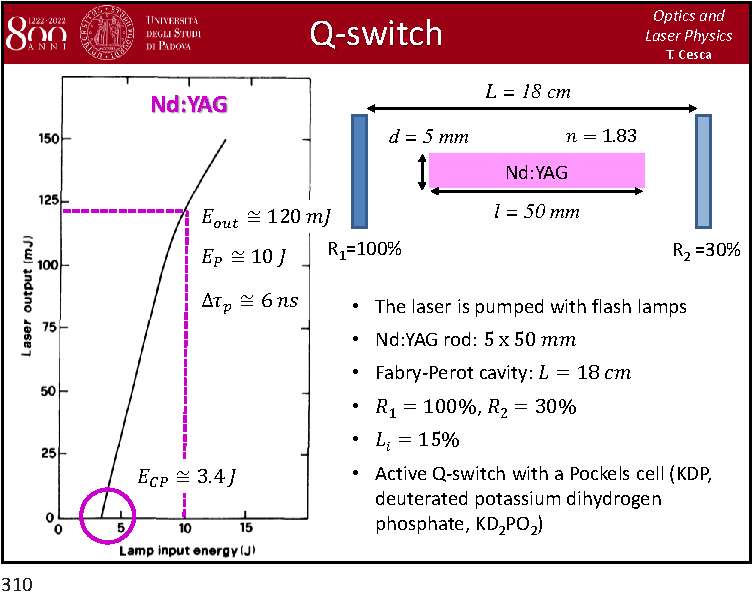
\includegraphics[page=1,width=1\textwidth]{../lessons/pdf_file/16_lecture.pdf}
\end{minipage}
\hspace{0.3cm}\vspace{0.3cm}
\begin{minipage}[c]{0.47\linewidth}

Let us compare the most relevant result for Q-switch with some experimental values for real system. We consider a Niudinium YAG laser and we have a pulse pumping.

Active Q-switch with a Pockels cell.

In the plot we see that there is a treshold energy.

\end{minipage}

\subsubsection*{Slide 2}

\begin{minipage}[]{0.5\linewidth}
\centering
\includegraphics[page=2,width=1\textwidth]{../lessons/pdf_file/16_lecture.pdf}
\end{minipage}
\hspace{0.3cm}\vspace{0.3cm}
\begin{minipage}[c]{0.47\linewidth}



\end{minipage}

\subsubsection*{Slide 3}

\begin{minipage}[]{0.5\linewidth}
\centering
\includegraphics[page=3,width=1\textwidth]{../lessons/pdf_file/16_lecture.pdf}
\end{minipage}
\hspace{0.3cm}\vspace{0.3cm}
\begin{minipage}[c]{0.47\linewidth}

From the graph, we can determine what is the utilization factor for a given threshold factor.

\end{minipage}

\newpage

\subsubsection*{Slide 4}

\begin{minipage}[]{0.5\linewidth}
\centering
\includegraphics[page=4,width=1\textwidth]{../lessons/pdf_file/16_lecture.pdf}
\end{minipage}
\hspace{0.3cm}\vspace{0.3cm}
\begin{minipage}[c]{0.47\linewidth}

Let us make an assumption that the mode is using entirely the active medium \( A_b \simeq A \). The stimulated emission cross section \( \sigma  \) is an intrinsic paramater of the material.

\end{minipage}

\subsubsection*{Slide 5}

\begin{minipage}[]{0.5\linewidth}
\centering
\includegraphics[page=5,width=1\textwidth]{../lessons/pdf_file/16_lecture.pdf}
\end{minipage}
\hspace{0.3cm}\vspace{0.3cm}
\begin{minipage}[c]{0.47\linewidth}

Theoretically we can determine a larger value than that what we can calculate experimentally. This is why:
\begin{itemize}
\item we assumed \( A_b \simeq A \), but in reality we have \( A_b < A \);
\item the fast switching time (one of the hypothesis) is much shorter than the build-up time..since the cavity is quite short, this condition cannot be satisfied. This means that we are wasting part of the energy of the pulse on the shutter itself because it take time to open.
\end{itemize}

\end{minipage}

\subsubsection*{Slide 6}

\begin{minipage}[]{0.5\linewidth}
\centering
\includegraphics[page=6,width=1\textwidth]{../lessons/pdf_file/16_lecture.pdf}
\end{minipage}
\hspace{0.3cm}\vspace{0.3cm}
\begin{minipage}[c]{0.47\linewidth}

We compute the pulse duration.
The losses are quite large and the lifetime photon is very small.

\end{minipage}

\newpage

\subsubsection*{Slide 7}

\begin{minipage}[]{0.5\linewidth}
\centering
\includegraphics[page=7,width=1\textwidth]{../lessons/pdf_file/16_lecture.pdf}
\end{minipage}
\hspace{0.3cm}\vspace{0.3cm}
\begin{minipage}[c]{0.47\linewidth}

As well in thi case we obtain a theoretical result which is smaller than the one we get experimentally.

We can make some hypothesis for these discrepancies:
\begin{itemize}
\item one of the working hypothesis is operating in single-mode oscillation, but if we do not do anything the system work in \textbf{multi-mode oscillation}. The build-up time is different for the different modes in the cavity... so we can have different gain for the different modes.

\item moreover, the fast-switching condition cannot be satisfied and this produce a broadening of the pulse.

\end{itemize}

\end{minipage}

\subsubsection*{Slide 8}

\begin{minipage}[]{0.5\linewidth}
\centering
\includegraphics[page=8,width=1\textwidth]{../lessons/pdf_file/16_lecture.pdf}
\end{minipage}
\hspace{0.3cm}\vspace{0.3cm}
\begin{minipage}[c]{0.47\linewidth}

Finally, let us compute the build-up time. Firstly, we compute the peak photon number.

We can assume that the volume of the mode of the active medium is \( V_a = A_b l \simeq A l \).

We have a very larger number of photons at the peak of the pulse.

The main reason for the discrepancy is that the build-up time is comparable with the times that it may take for swithing the element in the cavity.

However, this rate equation approach can catch up all the main results as the order of magnitude of the quantities.
It is a simple tool but powerful.

\end{minipage}

\subsubsection*{Slide 9}

\begin{minipage}[]{0.5\linewidth}
\centering
\includegraphics[page=9,width=1\textwidth]{../lessons/pdf_file/16_lecture.pdf}
\end{minipage}
\hspace{0.3cm}\vspace{0.3cm}
\begin{minipage}[c]{0.47\linewidth}

One of the working hypothesis to solve the rate equations was to operate in the \textbf{fast} Q-switch mode (the change in losses is considered to be instantaneous). The time of this transition is considered smalller than the build-up time to obtain photons in the cavity.

There is also the possibility to operate in the \textbf{slow} Q-switch mode in which we have a continuous decrease of the losses over time. In this case is possible to obtain a sequence of pulse: the gain factor which is proportional trough the stimulated emission cross section to the population of the active medium, and it is varying over time, if the losses decrease over time, we can get a situation in which the gain factor is larger than the losses at different moments (if the gain is larger than the losses means that you are able to obtain laser action).

\end{minipage}

The peak of the pulse will be smaller and smaller as the time goes on.

\subsubsection*{Slide 10}

\begin{minipage}[]{0.5\linewidth}
\centering
\includegraphics[page=10,width=1\textwidth]{../lessons/pdf_file/16_lecture.pdf}
\end{minipage}
\hspace{0.3cm}\vspace{0.3cm}
\begin{minipage}[c]{0.47\linewidth}

Before, we assumed the \textbf{pulsed pumping}. However, it is possible to operate in \textbf{continuous pumping} and repeat the Q-switching of the losses in the cavity. Again you can obtain multiple pulses which correspond to the time when the Q-switch is open. The rate equations are different in this case, the main is that when the first pulse is finish, we have that the initial population inversion is equal to the final population inversion that we get at the end of the previous pulse.

\end{minipage}

\subsubsection*{Slide 11}

\begin{minipage}[]{0.5\linewidth}
\centering
\includegraphics[page=11,width=1\textwidth]{../lessons/pdf_file/16_lecture.pdf}
\end{minipage}
\hspace{0.3cm}\vspace{0.3cm}
\begin{minipage}[c]{0.47\linewidth}

Let us make an exercise within the hypothesis of fast Q-switching and pulsing pumping.

\end{minipage}

\subsubsection*{Slide 12}

\begin{minipage}[]{0.5\linewidth}
\centering
\includegraphics[page=12,width=1\textwidth]{../lessons/pdf_file/16_lecture.pdf}
\end{minipage}
\hspace{0.3cm}\vspace{0.3cm}
\begin{minipage}[c]{0.47\linewidth}

\( \eta _E \) can be found graphically for the given threshold factor.

\end{minipage}

\subsubsection*{Slide 13}

\begin{minipage}[]{0.5\linewidth}
\centering
\includegraphics[page=13,width=1\textwidth]{../lessons/pdf_file/16_lecture.pdf}
\end{minipage}
\hspace{0.3cm}\vspace{0.3cm}
\begin{minipage}[c]{0.47\linewidth}



\end{minipage}

\subsubsection*{Slide 14}

\begin{minipage}[]{0.5\linewidth}
\centering
\includegraphics[page=14,width=1\textwidth]{../lessons/pdf_file/16_lecture.pdf}
\end{minipage}
\hspace{0.3cm}\vspace{0.3cm}
\begin{minipage}[c]{0.47\linewidth}



\end{minipage}

\subsubsection*{Slide 15}

\begin{minipage}[]{0.5\linewidth}
\centering
\includegraphics[page=15,width=1\textwidth]{../lessons/pdf_file/16_lecture.pdf}
\end{minipage}
\hspace{0.3cm}\vspace{0.3cm}
\begin{minipage}[c]{0.47\linewidth}



\end{minipage}

\subsubsection*{Slide 16}

\begin{minipage}[]{0.5\linewidth}
\centering
\includegraphics[page=16,width=1\textwidth]{../lessons/pdf_file/16_lecture.pdf}
\end{minipage}
\hspace{0.3cm}\vspace{0.3cm}
\begin{minipage}[c]{0.47\linewidth}



\end{minipage}

\subsubsection*{Slide 17}

\begin{minipage}[]{0.5\linewidth}
\centering
\includegraphics[page=17,width=1\textwidth]{../lessons/pdf_file/16_lecture.pdf}
\end{minipage}
\hspace{0.3cm}\vspace{0.3cm}
\begin{minipage}[c]{0.47\linewidth}

Let us see how to realize the \textbf{active Q-switching}. We can exploit the \textbf{electro-optic Kerr effect}: we can induce a difference in refractive index between two perpendicular components. When we apply a voltage to an isotropic material it is possible to obtain a difference in refractive index for the component parallel and perpendicular to the electric field. We take our material as birifringent and this difference in the refractive index is proportional to \( E^2 \). The proportionality is given by the \textbf{Kerr constant} \( K \): the larger it is, the smaller is the voltage that we need to apply to get the difference in refractive index.

\end{minipage}

Moreover, a difference in refractive index means a phase shift. In this way it is possible to realize a Cell in which applied by the outside a voltage and introducing a phase shift for two orthogonal component (it is useful for obtaining QWP or HWP).

Electro-optic Kerr cell are not used anymore for realizing thse cells.

\subsubsection*{Slide 18}

\begin{minipage}[]{0.5\linewidth}
\centering
\includegraphics[page=18,width=1\textwidth]{../lessons/pdf_file/16_lecture.pdf}
\end{minipage}
\hspace{0.3cm}\vspace{0.3cm}
\begin{minipage}[c]{0.47\linewidth}

Instead, the \textbf{Pockels effect} is used: we take a material and we place two electrods along the axis of the beam propagation (they need to be transparent!). The material used is a non-linear crystal and it could be already birifringence, it is possible to introduce \( \Delta n \) by appling an electric field along the direction \( z \).

\end{minipage}

\subsubsection*{Slide 19}

\begin{minipage}[]{0.5\linewidth}
\centering
\includegraphics[page=19,width=1\textwidth]{../lessons/pdf_file/16_lecture.pdf}
\end{minipage}
\hspace{0.3cm}\vspace{0.3cm}
\begin{minipage}[c]{0.47\linewidth}

The last can be used for an active shutter. PC is the pocket cell and it produce a shift of \( \pi /2 \).

Firstly we obtain circular polarization with the polarizer.
Each time a beam pass trough the Pockels cell it acquires a phase-shift of \( \pi /2 \).

The initial linear polarization is rotated of 90° and it will blocked by the polarizer. The shutter will be closed!

\end{minipage}

\subsubsection*{Slide 20}

\begin{minipage}[]{0.5\linewidth}
\centering
\includegraphics[page=20,width=1\textwidth]{../lessons/pdf_file/16_lecture.pdf}
\end{minipage}
\hspace{0.3cm}\vspace{0.3cm}
\begin{minipage}[c]{0.47\linewidth}

Another configuration used to prevent a reflected beam from entering along an optical pump is the so called \textbf{Faraday rotator}.

When you apply a magnetic field \( B \) and you are travelling trough the material with size \( d \), the linear polarization of the beam is rotated of \( \beta  \).

If the beam is reflected back and it pass again trough the material, since the rotation is independent on the direction of propagation within the material,
the beam rotate again by \( \beta  \).
At the end the beam will arrive rotating at 90°, so it will be blocked by a linear polarizer.

\end{minipage}

\subsubsection*{Slide 21}

\begin{minipage}[]{0.5\linewidth}
\centering
\includegraphics[page=21,width=1\textwidth]{../lessons/pdf_file/16_lecture.pdf}
\includegraphics[page=22,width=1\textwidth]{../lessons/pdf_file/16_lecture.pdf}
\end{minipage}
\hspace{0.3cm}\vspace{0.3cm}
\begin{minipage}[c]{0.47\linewidth}

This is an example to see how the Pockels cell can be used. We can realize a \textbf{pulse slicer}: device used to select a pulse between a train of pulses.

It is composed by a linear polarizer, a first PC, an HWP, a second PC and another polarizer.

At the begin we suppose that PC1 and PC2 are off. The second polarizer will see a beam with a polarization of -45° (the HWP flip the polarization at -45°) and the beam will be blocked.

If PC1 is on and PC2 off and if PC1 behave as an HWP, we have first a flip of 45° by the Pol1, then the PC1 flips at -45°, HWP flips to 45° and at the end you will enter to the Pol2 at 45°. You will obtain a beam out.

If PC1 and PC2 are both on, you will get any beam outside.


\end{minipage}

\end{document}
